%%%%%%%%%%%%%%%%%%%%%%%%%%%%%%%%%%%%%%%%%
% LaTeX Template
%%%%%%%%%%%%%%%%%%%%%%%%%%%%%%%%%%%%%%%%%

%----------------------------------------------------------------------------------------
%	PACKAGES AND DOCUMENT CONFIGURATIONS
%----------------------------------------------------------------------------------------

\documentclass[twoside,a4paper]{article}
\usepackage{geometry}

\usepackage{siunitx} % Provides the \SI{}{} and \si{} command for typesetting SI units
\usepackage{graphicx} % Required for the inclusion of images
\usepackage[square,sort,comma,numbers]{natbib}
\usepackage{amsmath} % Required for some math elements
\usepackage{lastpage} % know last page (used in fancy header)
\usepackage{fancyhdr} % Fancy Header
\usepackage[xindy, toc, numberedsection]{glossaries} % glossaries with xindy (recommended) for the indexing phase and show glossaries in TOC, and numberedsection to get a Setion number in the title
\usepackage{url} %The command is intended for email addresses, hypertext links, directories/paths, etc., which normally have no spaces, so by default the package ignores spaces in its argument.
\usepackage{minted} % it allows formatting and highlighting source code
% in addition, Pygments must be installed
% How to install on Windows:
% 1) install python (and add it to your PATH)
% 2) install pip (https://pip.pypa.io/en/stable/installing/)
% 3) install pygments (pip install Pygments)
% add pygments to your PATH, the command "pip show Pygments" shows where the lib is installed
% Of course, pdfLaTeX (or whatever engine/format you use) still has to be called with the -shell-escape option.



\loadglsentries{glossaries.tex}
\makeglossaries % generate the glossary
% Any links in resulting glossary will not be "clickable" unless you load the glossaries package after the hyperref package.

\setlength\parindent{0pt} % Removes all indentation from paragraphs

\renewcommand{\labelenumi}{\alph{enumi}.} % Make numbering in the enumerate environment by letter rather than number (e.g. section 6)

\renewcommand{\arraystretch}{1.2} % Increasing the array stretch factor using \renewcommand{\arraystretch}{<factor>} where <factor> is a numeric value

%\usepackage{times} % Uncomment to use the Times New Roman font

%----------------------------------------------------------------------------------------
%	DOCUMENT INFORMATION
%----------------------------------------------------------------------------------------
\newcommand{\maintitle}{ADD - INVERT}
\newcommand{\course}{Labo Geavanceerde Computertechniek}
\newcommand{\coursenumber}{JLIZNM}
\newcommand{\class}{MELICTEES}

%%%%%%%%%%%%%%%%%%%%%%%%%%%%%% HEADER %%%%%%%%%%%%%%%%%%%%%%%%%%%%%%
\pagestyle{fancy}
\fancyhf{}
\fancyhead[LE,RO]{\course}
\fancyhead[RE,LO]{\maintitle}
% if working with chapters
% \fancyfoot[CE,CO]{\leftmark}
\fancyfoot[LE,RO]{\thepage\ of \pageref{LastPage}}
%%%%%%%%%%%%%%%%%%%%%%%%%%%%%% HEADER %%%%%%%%%%%%%%%%%%%%%%%%%%%%%%


%%------------------------------ TITLE PAGE -----------------------------
\title{\maintitle \\ \course \\{\small\ (\coursenumber)}} % Title

\author{Jona \textsc{Cappelle} \& \textsc{Jonas Bolle}} % Author name

\date{\today} % Date for the report

\begin{document}\sloppy % sloppy is used to enforce that lines are in hbox
\newgeometry{hmarginratio=1:1}    %% make layout symmetric
\pagenumbering{gobble}% Remove page numbers (and reset to 1)
\begin{titlepage}
\maketitle % Insert the title, author and date

\vfill
\begin{center}

\includegraphics[width=0.13\textwidth]{logo_kuleuven.png} %
\end{center}
%each \vfill will expand vertically the same amount until the entire page is filled
\vfill
\vfill
\vfill

\begin{center}
\begin{tabular}{l r}
Session Date: & January 1, 2017 \\ % Date the experiment was performed
\\
Partners: &  Jona Cappelle\\ % Partner names
&  Jonas Bolle\\
Class: & \class \\
\\
Instructor: &  Stijn Crul% Instructor/supervisor
\end{tabular}
\end{center}
\vfill
\vfill
\end{titlepage}
\clearpage
\newpage\null\thispagestyle{empty}\newpage % blank page after title page

%%------------------------------ TITLE PAGE -----------------------------


\restoregeometry%              %% restore the layout
\pagenumbering{arabic}% Arabic page numbers (and reset to 1)

\tableofcontents
\listoffigures
\listoftables
\listoflistings%
\clearpage

%----------------------------------------------------------------------------------------
%	INLEIDING
%----------------------------------------------------------------------------------------
\section{Inleiding}
In dit eerste labo geavanceerde computerarchitectuur maken we kennis met CUDA, een extensie van de C programmeertaal gemaakt door nVidia. Het grote voordeel hierbij is dat de code op de GPU kan uitgevoerd worden. Hierdoor kan de programmeur gebruik maken van de zeer grote parallele rekenkracht van een nVidia grafische kaart. Cuda is enkel geschikt voor algoritmes die geparalleliseerd kunnen worden.

In dit eerste labo gaan we twee kleine cuda programmaatjes schrijven. Het eerste is om twee arrays op te tellen, het tweede is om een arrray te inverteren.
\cite{whatiscuda}

De architectuur van een CPU en GPU verschilt drastisch (zie figuur \ref{fig:cpugpu}).
\begin{figure}[H]
    \centering
    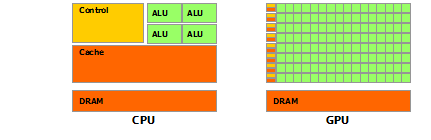
\includegraphics[scale=0.7]{gpu-devotes-more-transistors-to-data-processing.png}
    \caption{Vergelijking architectuur CPU vs GPU \cite{cudaprogrammingguide}}
    \label{fig:cpugpu}
\end{figure}

Een GPU bestaat uit grids, blocks en threads. Een grid bestaat uit verschillende blocks, die op zijn beurt bestaat uit verschillende threads. Nu is het aan de programmeur om deze threads op zo'n efficient mogelijke manier te gebruiken.
\cite{cudaprogrammingguide}

\begin{figure}[H]
    \centering
    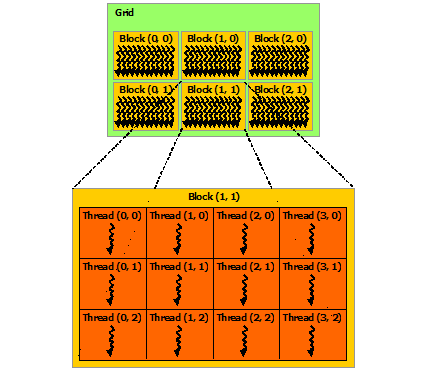
\includegraphics[scale=0.6]{grid-of-thread-blocks.png}
    \caption{Grids, blocks en threads \cite{cudaprogrammingguide}}
    \label{fig:gridthreadblocks}
\end{figure}

%----------------------------------------------------------------------------------------
%	PROBLEEMSTELLING
%----------------------------------------------------------------------------------------
\section{Probleemstelling}
We zullen in dit labo twee arrays optellen en een array inverteren. We zullen dit een aantal keren doen. De timing om al deze operaties uit te voeren zal opgenomen worden, dit zowel op de GPU als op de CPU. Hieruit zullen we laten conclusies kunnen trekken. We onderzoeken ook de invloed van de blocksize op de GPU. De operaties op de GPU zullen getimed worden met het copi\"eren van data naar de GPU en terug en zonder het copi\"eren van de data.

% welke uitdagingen
% wat wordt er onderzocht

%----------------------------------------------------------------------------------------
%	OPLOSSING
%----------------------------------------------------------------------------------------
\section{Oplossing}

\subsection{Flowchart code}

\begin{figure}[H]
    \centering
    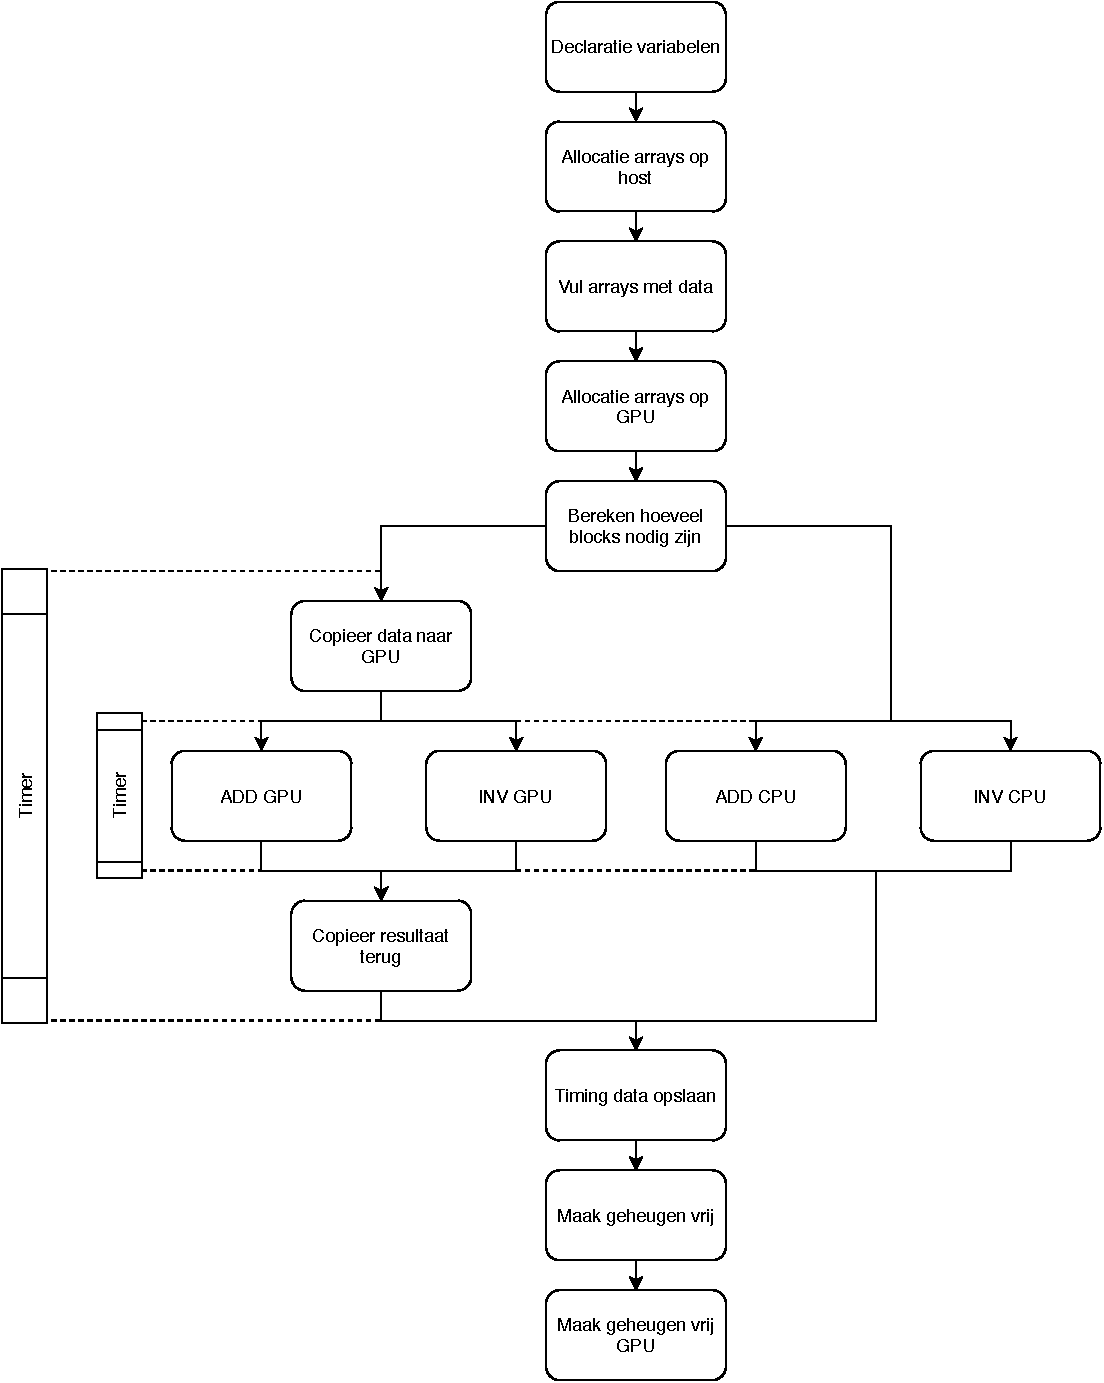
\includegraphics[width=\columnwidth]{flowchart_inv_add.pdf}
    \caption{Flowchart ADD - INV}
    \label{fig:flowchart}
\end{figure}

\subsection{Code}
De volledige cuda code kan u terug vinden in bijlage \ref{code} op pagina \pageref{code}.

%----------------------------------------------------------------------------------------
%	ANALYSE PERFORMANTIE
%----------------------------------------------------------------------------------------
\section{Analyse performantie}

\subsection{Tijd op CPU}

\subsection{Tijd op GPU}


%----------------------------------------------------------------------------------------
%	BESLUIT
%----------------------------------------------------------------------------------------
\section{Besluit}
% waarom goed / niet goed



\newpage
\appendix
\section{CODE}
\label{code}
\inputminted[linenos=true, breaklines=true]{cuda}{template.cu}

%----------------------------------------------------------------------------------------
%	BIBLIOGRAPHY
%----------------------------------------------------------------------------------------
\clearpage
\bibliographystyle{IEEEtranN}
\bibliography{bib}

%----------------------------------------------------------------------------------------

\end{document}